\section{Third- versus fourth-order property-mode experiment (E9)}
\label{sec:S_e9}

\subsection{Frozen protocol and metric correction}
E9 was frozen after the earlier E8 RMSE result was known but before any new E9 outer metric was computed. The preregistration and machine-readable protocol are \path{E9_PREREGISTRATION.md} and \path{studies/brugge_sparse_sensing/e9_protocol.json}; their SHA-256 values are stored in every fold selection record. Ten P2 leave-one-scenario-out folds use three deterministic scenario-grouped inner folds and all 133 report steps only once for the final outer evaluation. Inner selection balances the mean property-wise anomaly-relative error and anomaly DSSIM. The same measurement rows, report steps and one pairwise common inner-selected LS/ridge solver are applied to each 3D--4D comparison. LASSO is a declared frozen-final sensitivity and cannot select a reported model.

\begin{table}[htbp]
\centering
\scriptsize
\caption{Historical metric intent, implementation problem and E9 correction.}
\label{tab:S_e9_metrics}
\begin{tabular}{@{}p{0.22\linewidth}p{0.34\linewidth}p{0.35\linewidth}@{}}
\toprule
Original metric & Audited problem & E9 use \\
\midrule
Relative Frobenius error & Large pressure datum dilutes scenario-specific error; historical call also included inactive cells and rounded estimates & Property-wise physical residual divided by the held-out anomaly norm; raw relative error retained as sensitivity \\
SSIM & Inactive background entered rectangular windows; swapped arguments; non-standard constants; implementation disagreed with the text & Gaussian local moments renormalised over active cells; active-centred windows with at least half active in-domain weight; train-only anomaly range \\
RMSE & Valid physical-unit score but cannot alone compare two differently scaled properties or structure & Mandatory auxiliary endpoint, never removed when it disagrees with anomaly error or SSIM \\
PSNR & Monotone transformation of MSE under fixed range & Omitted \\
\bottomrule
\end{tabular}
\end{table}

Raw-field SSIM is diagnostically saturated: optimized outer records have median scores near one for both properties, while anomaly SSIM spans a broad range and gives materially larger 3D--4D separation. Unit tests establish identity, symmetry, determinism, inactive-background invariance, invalid-window handling, vectorised equivalence and train-only reference fitting.

\subsection{Dependence and property rank}
Figure~\ref{fig:S_e9_coupling} reports dependence using outer-training scenarios only. Cell/time anomalies have correlation \ENineAnomalyCorrelation, but spatial-mean anomaly trajectories correlate at \ENineTemporalCorrelation. Leading spatial subspaces are partly aligned (mean top-16 cosine \ENineSubspaceAlignment) and the leading standardised property direction contains \ENineRankOneEnergy{} of property-mode energy. This combination supports partial sharing and explains why property rank one is not selected. Exploratory fold-level coupling--gain correlations have inconsistent signs across budgets and none survives false-discovery-rate control; they do not establish a causal coupling threshold.

\begin{figure}[htbp]
\centering
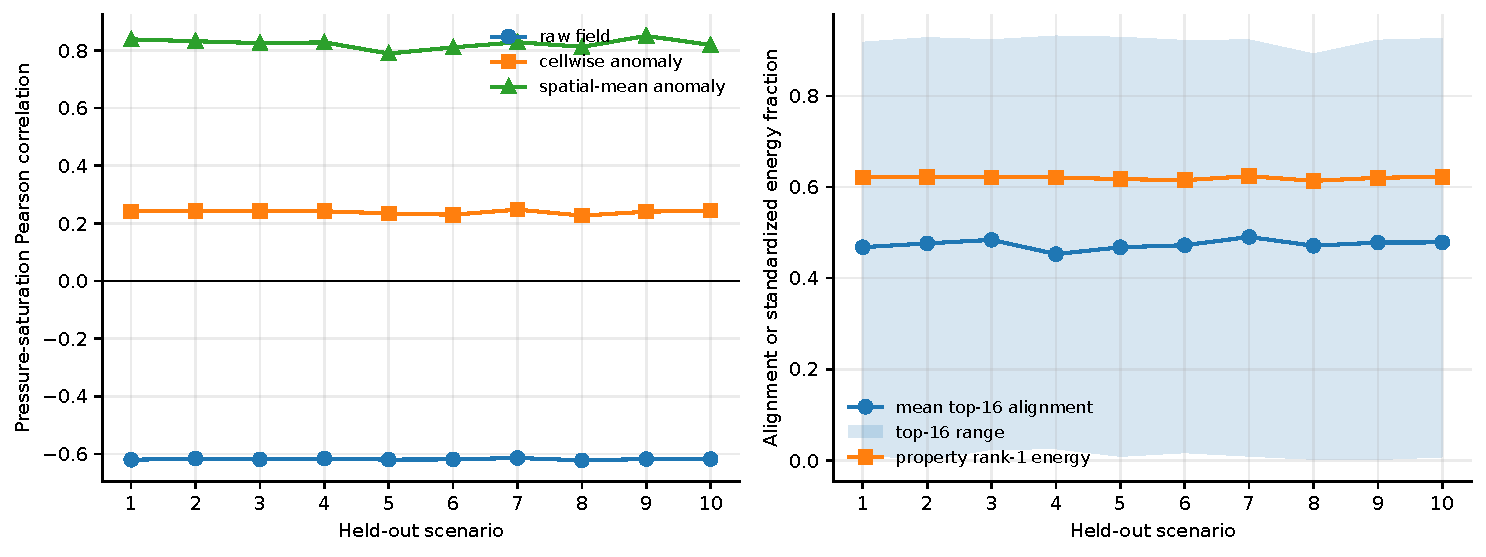
\includegraphics[width=\textwidth]{../../../../studies/brugge_sparse_sensing/figures/fig17_e9_cross_property.pdf}
\caption{Train-only pressure--saturation dependence by held-out scenario. Left: raw, cellwise-anomaly and spatial-mean-anomaly correlations. Right: leading spatial-subspace alignment and the standardised property rank-one energy.}
\label{fig:S_e9_coupling}
\end{figure}

\subsection{Architectures, capacity and ablation}
Independent 3D fits separate space--space--time tensors. 4D-A shares spatial/property factors and coefficients; 4D-B shares spatial factors but not property coefficients; 4D-C weights the joint objective; 4D-D adds property-specific spatial factors; 4D-E adds property-specific tensor residual modes. Equal-total capacity compares 16+16 independent coefficients with 32 fourth-order coefficients; equal-per-property compares 32+32 with 64. Property rank one/two, spatial ranks, anomaly treatment and weighting are selected inside each outer-training fold.

Figure~\ref{fig:S_e9_ablation} reports all fourth-order variants at the prespecified 15-well equal-total slice. Each variant has its own train-only representation and the pairwise common solver selected with independent 3D; the figure does not retrospectively choose the best outer variant. Across the complete selection, 4D-B is chosen in \ENineSharedHeadSelections{} of \ENineSparseSelections{} sparse comparisons and every full-observation comparison. Weighted and residual variants help in individual folds, especially at five wells, but are not stable global winners. The rigid current model meets the headline advantage rule only \ENineCurrentAdvantages{} times; optimization meets it \ENineHeadlineAdvantages{} times out of \ENineHeadlineComparisons.

\begin{figure}[htbp]
\centering
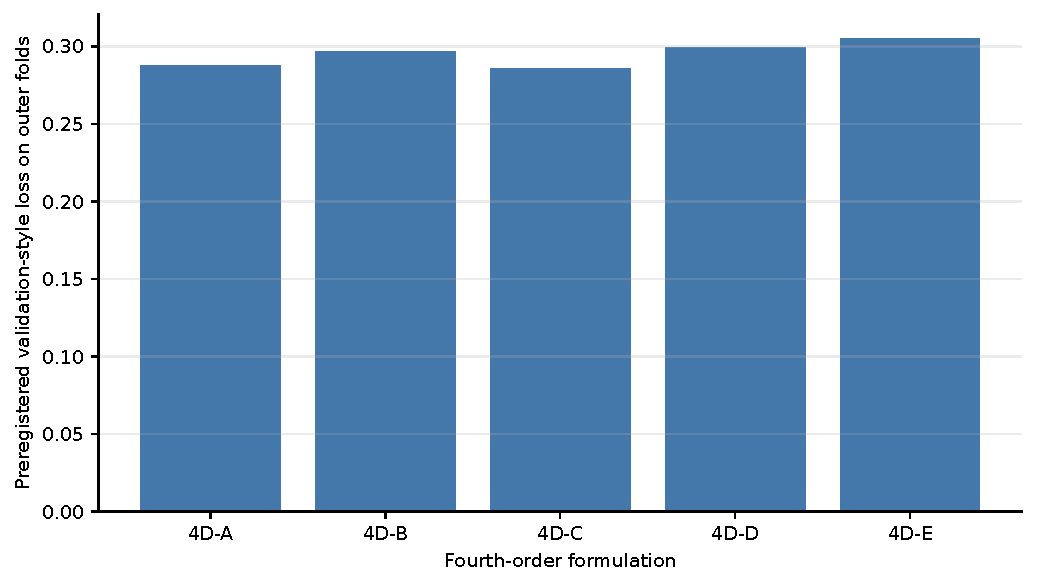
\includegraphics[width=0.82\textwidth]{../../../../studies/brugge_sparse_sensing/figures/fig18_e9_ablation.pdf}
\caption{Fourth-order architecture ablation at 15 configured wells and equal-total capacity. The displayed outer score has the same error/DSSIM form as the frozen validation objective, but outer values never feed selection. Lower is better.}
\label{fig:S_e9_ablation}
\end{figure}

\subsection{Complete evidence and interpretation}
The canonical files \path{outer_selected_results.csv}, \path{outer_summary.csv} and \path{paired_comparisons.csv} contain every fold value, mean, median, SD, IQR, signed paired difference and descriptive Wilcoxon result. \path{selected_configuration_frequency.csv} records fold-specific architectures, transforms, ranks and common solvers. \path{metric_ranking_audit.csv} identifies the \ENineRankingDifferences{} metric-discordant property/regime comparisons rather than collapsing them to one winner. The fixed map metadata are in \path{representative_map_metrics.json}.

The frozen-final LASSO sensitivity contains 320 outer records at the declared $\lambda=10^{-3}$. Raising only the iteration ceiling from 5,000 to 20,000 after the first convergence diagnostic still leaves 50 fits at the ceiling. LASSO favours 4D by the directional fold rule in 49 of 64 regime/metric comparisons, but the unconverged subset makes this supportive rather than confirmatory evidence. No LASSO value enters selection or the headline LS/ridge conclusions; iterations and all failed-to-converge-at-ceiling fits remain visible in \path{lasso_sensitivity.csv}.

The evidence supports shared spatial-factor estimation with independent property heads, especially under severe undersampling. It does not support universal fourth-order superiority, rigid shared coefficients, property rank-one compression, or a full-state saturation gain. E8 therefore remains a valid negative result for the original formulation; E9 explains the limitation and identifies the narrower regime in which a property mode is useful.

% Generated by e9_analyze.py; do not edit.
\begin{table*}[htbp]\centering\small
\caption{E9 equal-total-capacity diagnostic scores and mean factor/core storage (float entries). Pressure RMSE uses the supplied export unit $u_p$; oil-saturation RMSE is dimensionless. Budget counts scalar channels for grid sensing and two-property wells for well sensing. Values are mean $\pm$ sample standard deviation over ten outer scenarios. 3D and 4D denote the independently train-selected models.}
\label{tab:e9_diagnostics}
\setlength{\tabcolsep}{3pt}
\begin{adjustbox}{max width=\textwidth}
\begin{tabular}{lrlrrr}\toprule
Geometry & Budget & Model & RMSE$_p$ & RMSE$_{S_o}$ & Stored floats \\ \midrule
grid & 30 & 3D & 1.166 $\pm$ 0.294 & 0.0008 $\pm$ 0.0003 & 149728 \\
grid & 30 & 4D & 0.372 $\pm$ 0.137 & 0.0004 $\pm$ 0.0001 & 141674 \\
grid & 300 & 3D & 0.147 $\pm$ 0.032 & 0.0003 $\pm$ 0.0001 & 149728 \\
grid & 300 & 4D & 0.102 $\pm$ 0.029 & 0.0003 $\pm$ 0.0001 & 155098 \\
wells & 5 & 3D & 0.486 $\pm$ 0.088 & 0.0018 $\pm$ 0.0002 & 149728 \\
wells & 5 & 4D & 0.411 $\pm$ 0.144 & 0.0009 $\pm$ 0.0002 & 180450 \\
wells & 15 & 3D & 0.210 $\pm$ 0.049 & 0.0010 $\pm$ 0.0002 & 149728 \\
wells & 15 & 4D & 0.216 $\pm$ 0.077 & 0.0008 $\pm$ 0.0003 & 160881 \\
wells & 30 & 3D & 0.189 $\pm$ 0.083 & 0.0007 $\pm$ 0.0002 & 149728 \\
wells & 30 & 4D & 0.121 $\pm$ 0.055 & 0.0007 $\pm$ 0.0003 & 153962 \\
\bottomrule\end{tabular}
\end{adjustbox}
\end{table*}


\subsection{Exact structural metric}
For an active window centre $c$, let $g_{ca}$ be the Gaussian weight of in-domain cell $a$, $m_a$ the binary active mask, and $w_{ca}=g_{ca}m_a/\sum_b g_{cb}m_b$. Windows require $\sum_a g_{ca}m_a/\sum_a g_{ca}\geq 1/2$. For true and reconstructed anomalies $x_a,y_a$, define $\mu_x=\sum_a w_{ca}x_a$, $\mu_y=\sum_a w_{ca}y_a$, $v_x=\max(\sum_a w_{ca}x_a^2-\mu_x^2,0)$, $v_y$ analogously, and $v_{xy}=\sum_a w_{ca}x_ay_a-\mu_x\mu_y$. Then
\begin{equation}
\operatorname{SSIM}'_c=\frac{(2\mu_x\mu_y+C_1)(2v_{xy}+C_2)}{(\mu_x^2+\mu_y^2+C_1)(v_x+v_y+C_2)},\qquad C_j=(K_j L_k)^2.
\label{eq:S_ssim}
\end{equation}
Here $L_k$ is the training-anomaly range for property $k$, $K_1=0.01$ and $K_2=0.03$. Equation~\eqref{eq:S_ssim} uses population moments; no sample-covariance correction is applied. Zero padding carries zero domain weight. The implementation averages valid centres and report steps equally. A zero anomaly range falls back to the raw training range; a zero raw range is rejected. A zero anomaly-error denominator gives zero only for exact reconstruction and infinity otherwise. None of these degenerate cases occurs in the retained outer results.
